\chapter{Two level system (Landau-Zener)}
\textit{\today\newline
Jan Střeleček\newline}




Let's have a Hamiltonian
\begin{equation}
    \HH(t)=\begin{pmatrix}
        \Omega(t)&\Delta(t)\\
        \Delta(t)&-\Omega(t)
    \end{pmatrix}
\end{equation}
for $\Omega: \R^+\rightarrow \R$, $\Delta: \R^+\rightarrow \R$. Its spectrum is
\begin{equation}
    E_1(t)=-E_0(t)= \sqrt{\Omega^2(t)+\Delta^2(t)}
    \label{eq:energy}
\end{equation}
and eigenvectors
\begin{equation}
\ket{0(t)}=N_+ \begin{pmatrix}
 \frac{E_0(t)+\Omega(t)}{\Delta(t)} \\ 1
\end{pmatrix};\quad \ket{1(t)}=N_-\begin{pmatrix}
    \frac{E_1(t)+\Omega(t)}{\Delta(t)} \\ 1
   \end{pmatrix}
   \label{eq:eigenvectors}
\end{equation}
for normalization constants $N_\pm=\left(\left(\frac{\pm E_0(t)+\Omega(t)}{\Delta(t)}\right)^2+1\right)^{-1/2}$.

The goal will be to find \emph{fidelity} $F\coloneqq |\braket{0(t)|\psi(t)}|^2$ of different driving protocols. For this we need to solve time Schr\"odinger equation
\begin{equation}
    \HH(t)\ket{\psi(t)}=i\frac{\d}{\d t}\ket{\psi(t)}
\end{equation}
with time varying Hamiltonian. For 2-dimentional system with $\ket{\psi(t)}\eqqcolon (a(t),b(t))$ we get the system of \emph{two coupled differentials equations of the 1. order with non-constant coefficients}
\begin{align}
    \Omega(t)a(t)+\Delta(t)b(t)&=i\dot a(t)\label{eq:a1}\\
    \Delta(t)a(t)-\Omega(t)b(t)&=i\dot b(t)
    \label{eq:a2}
\end{align}
with normalization
\begin{equation}
    a^2(t)+b^2(t)=1, \quad \forall t\in [0,T_f].
    \label{eq:normalizationCondition}
\end{equation}
and initial value 
\begin{equation}
    \begin{pmatrix}
        a(0)\\b(0)
    \end{pmatrix} = \ket{0(0)}.
\end{equation}

\subsection{Harmonic oscillator correspondence}
The Equations \ref{eq:a1}, \ref{eq:a2} have no general analytical solution, with exceptions of a few easy protocols $\HH(t)$. Still we can find some general behavior. 

N-dimensional Schr\"odinger equation can be rewritten to \emph{one differential equation of N$^{th}$ order with non-constant coefficients}. In our two dimensional case, this equation corresponds to \emph{damped harmonic oscillator without external force}
\begin{align}
    0&= \ddot a(t)+ \gamma(t) \dot a(t)+\omega^2(t)a(t) \label{eq:harmonicOscillator}\\
    \gamma(t)&\coloneqq -\frac{\dot \Delta(t)}{\Delta(t)} \label{eq:gammaDef}\\
    \omega^2(t) &\coloneqq i\left(\dot \Omega(t)-\frac{\dot\Delta(t)}{\Delta(t)}\Omega(t)\right)+\Delta^2(t)+\Omega^2(t).
    \label{eq:frequency}
\end{align}
Along with normalization condition \ref{eq:normalizationCondition} and initial conditions
\begin{equation}
    \begin{pmatrix}
        a(0)\\b(0)
    \end{pmatrix}=\ket{0(t)}; \quad \dot a(0)=-i\left(\Omega(0) a(0)+\Delta(0)b(0)\right).
\end{equation}
Note that in this form $\Delta\neq 0$. This is not problem due to system symmetry $\Delta\leftrightarrow \Omega$, which means we can change the driving by interchanging $\Delta$ and $\Omega$ on any problematic intervals.


\subsubsection{Classical mechanics correspondence}
From the perspective of classical mechanics, meaning $x(t)\coloneqq a(t)$ is a position in a phase space $(\bm x,\bm p)$, we can write classical Lagrangian from Eq. \ref{eq:harmonicOscillator} as
\begin{equation}
    \mathcal L=\frac{1}{2}\exp{\left(\int_0^t\gamma(s)\d s\right)}\left(\dot x^2-\omega^2(t)x^2\right)
    \label{eq:lagrangian}
\end{equation}
\begin{proof}
    The correspondence of Lagrangian \ref{eq:lagrangian} with Eq. \ref{eq:harmonicOscillator} can be shown by direct evaluation of Euler-Lagrange equations
    \begin{equation}
        \begin{split}
            \pder{\mathcal L}{x}-\der{}{t}\pder{\mathcal L}{\dot x}&=0\\
            \frac{1}{2}\exp{\left(\int_0^t\gamma(s)\d s\right)}(-2 \omega^2(t)x)-\der{}{t}\left(\exp{\left(\int_0^t\gamma(s)\d s\right)}\dot x\right) &=0\\
            -\omega^2(t)x-\gamma(t)\dot x-\ddot x&=0,
        \end{split}
    \end{equation}
    where derivation along upper bound $F(x)\coloneqq\int_0^{g(x)}f(t)\d t \Rightarrow F'(x)=f(g(x))g'(x)$ for $f(t)\in L^1(0,g(x))$ and differentiable function $g$, was used.
\end{proof}


\section{Geodesical driving}
As was mentioned, the \Schrodinger equation has no general analytical solution, except a few easy protocols $\HH(t)$. One of them is \emph{Geodesical protocol}. 

Define driving in 3-dimensional space (the reason will be the urge to rewrite it using $\hat\sigma$ matrices)
\begin{equation}
    d(t)\equiv \begin{pmatrix}
        \Omega(t)\\
        \Xi(t)\\
        \Delta(t)
    \end{pmatrix}\coloneqq \begin{pmatrix}
        -s \cos(\omega(T_f)t)\\
        0\\
        s \sin(\omega(T_f)t)
    \end{pmatrix}
\end{equation}
parametrized by time $t\in[0,1]$ and with use of \emph{speed regulating function} $\omega(T_f)\coloneqq \pi/T_f$. This means, the driving will always be along half-sphere, as in Fig. \ref{fig:driving}.

\begin{figure}[H]
    \centering
    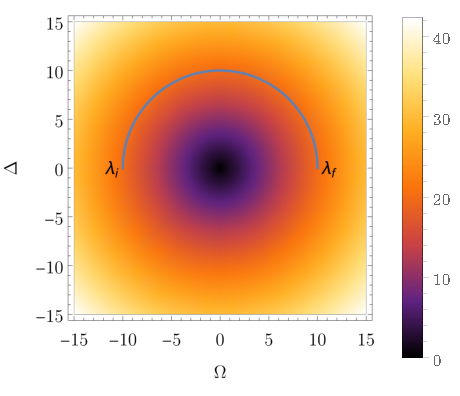
\includegraphics[scale=1.2]{../img/driving.pdf}
    \caption{Driving along the geodesic. $\lambda_i$ and $\lambda_f$ are initial resp. final parameters. DensityPlot shows the difference between Hamiltonian eigenvalues.}
    \label{fig:driving}
\end{figure}

\subsection{Derivation of the fidelity}
Because the Hamiltonian can be rewritten using Pauli matrices
\begin{equation}
    \HH(t) = 
        \begin{pmatrix}
         -s \cos (t \omega ) & s \sin (t \omega ) \\
         s \sin (t \omega ) & s \cos (t \omega ) \\
        \end{pmatrix}
        =\Delta(t)\sigma_x+ \Omega(t)\sigma_z= d(t).\mathbf{\hat\sigma}
\end{equation}
one can see that changing from the \textcolor{purple}{original frame} to \textcolor{blue}{moving frame of reference} (let's omit the final time dependence $\omega=\omega(T_f)$ for a while) 
\begin{equation}
    \textcolor{purple}{\psi(t)} \eqqcolon \expsp \textcolor{blue}{\tilde\psi(t)}
\end{equation}
reflects rotational symmetry of the problem. This change of reference frame transforms Schr\"odinger equation
\begin{equation}
    \begin{split}
        \textcolor{purple}{\HH(t)\psi(t)} &= i\textcolor{purple}{\psi'(t)}\\
        \textcolor{purple}{\HH(t)} \expsp\textcolor{blue}{\tilde\psi(t)} &= i \expsp \left(\frac{i\omega\hat\sigma_y}{2}\right)\textcolor{blue}{\tilde\psi(t)}+i\expsp\textcolor{blue}{\tilde\psi'(t)}\\
        \underbrace{\left(\expsm \textcolor{purple}{\HH(t)}\expsp+ \frac{\omega}{2}\hat\sigma_y\right)}_{\textcolor{blue}{\tilde\HH(t)}}\textcolor{blue}{\tilde\psi(t)}&=i\textcolor{blue}{\tilde\psi'(t)}.
    \end{split}
\end{equation}
Therefore we can equivalently solve the Fidelity problem in this new coordinate system.

Hamiltonian in the moving frame is
\begin{equation}
    \textcolor{blue}{\tilde\HH}=\textcolor{blue}{\begin{pmatrix}
        -s&-i\omega(T_f)/2\\
        i\omega(T_f)/2&s
    \end{pmatrix}},
\end{equation}
which is time independent. The Schr\"odinger equation can now be easily solved using evolution operator
\begin{equation}
    \begin{split}
        \textcolor{blue}{\UU(t)}=&e^{-i\textcolor{blue}{\tilde\HH}t}\\
        =&\textcolor{blue}{\begin{pmatrix}
            \cos \left(\frac{t}{2} q(T_f)\right)+\frac{2 i s \sin \left(\frac{t}{2} q(T_f)\right)}{q(T_f)} & -\frac{\omega(T_f)  \sin \left(\frac{t}{2} q(T_f)\right)}{q(T_f)} \\
            \frac{\omega(T_f)  \sin \left(\frac{t}{2} q(T_f)\right)}{q(T_f)} & \cos \left(\frac{t}{2} q(T_f)\right)-\frac{2 i s \sin \left(\frac{t}{2} q(T_f)\right)}{q(T_f)} \\
        \end{pmatrix}},
    \end{split}
    \label{eq:evolutionBlue}
\end{equation}
for $q(T_f)=\sqrt{4 s^2+\omega(T_f) ^2}$.

In the original frame we get the evolution of the state $\psi(0)$
\begin{equation}
    \textcolor{purple}{\psi(t)}=\expsp \textcolor{blue}{\UU(t) \tilde\psi(0)} = \underbrace{\expsp \textcolor{blue}{\UU}\expsm}_{\textcolor{purple}{\UU(t)}} \underbrace{\expsp \textcolor{blue}{\tilde\psi(0)}}_{\textcolor{purple}{\psi(0)}}.
\end{equation}
Then the evolved wavefunction is
\begin{equation}
    \textcolor{purple}{\ket{\psi(t)}}=\textcolor{purple}{\begin{pmatrix}
        \cos \left(\frac{t}{2} q(T_f)\right)+\frac{2 i s \cos (t \omega(T_f) ) \sin \left(\frac{t}{2} q(T_f)\right)}{q(T_f)}\\
        \frac{(\omega(T_f) -2 i s \sin (t \omega(T_f) )) \sin \left(\frac{t}{2} q(T_f)\right)}{q(T_f)}
    \end{pmatrix}}
\end{equation}
and the ground state
\begin{equation}
    \textcolor{purple}{\ket{0(t)}}=\textcolor{purple}{\mathcal{N}\begin{pmatrix}
        -\cot (\frac{t}{2}\omega(T_f))\\
        1
    \end{pmatrix}},
\end{equation}
for a normalization constant $\textcolor{purple}{\mathcal{N}}\coloneqq |\textcolor{purple}{\braket{0(t)|0(t)}}|^{-1}$.
Fidelity during the transport is then\footnote{If we would calculate the fidelity in the \textcolor{blue}{comoving frame}, we would get exactly one. This is the essence of counterdiabatic driving.}
\begin{equation}
    F=\left|\textcolor{purple}{\braket{0(t)|\psi(t)}}\right|^2,
    \label{fid:definition}
\end{equation}

 An explicit formula for fidelity in time $t$ and geodesic driving with final time $T_f$ is then
\begin{equation}
    F(t,T_f)=\frac{\pi ^2 \left(\cos \left(t \sqrt{\frac{\pi ^2}{T_f^2}+4 s^2}\right)+1\right)+8 s^2 T_f^2}{2 \sin ^4\left(\frac{\pi  t}{2 T_f}\right) \left(4 s^2 T_f^2+\pi ^2\right) \left(\left| \cot \left(\frac{\pi  t}{2 T_f}\right)\right|^2+1\right)^2}.
    \label{eq:fidelitySimplified}
\end{equation}
The domain can be extended to $t\in[0,T_f]$, $T_f\in[0,\infty]$ because 
$$
    \lim_{t\rightarrow 0}F=1\; ,\;\; \lim_{T_f\rightarrow 0}F=0.
$$

Sometimes the \emph{Infidelity}, defined as $I\coloneqq 1-F$, will be used. Its meaning is \emph{the probability of excitation of the state}.


\subsection{Analysis of the infidelity formula}
Fidelity for some fixed final time is just oscilating curve close to $1$. For $T_f=10$ it can be seen on Fig. \ref{fig:infidelityTimePlot}. The \emph{final fidelity} (at $t=T_f$) dependence on final time $T_f$ can be seen on Fig. \ref{fig:infidelityTfPlot} and \ref{fig:infidelityTfPlotLog}.
\begin{figure}[H]
    \centering
    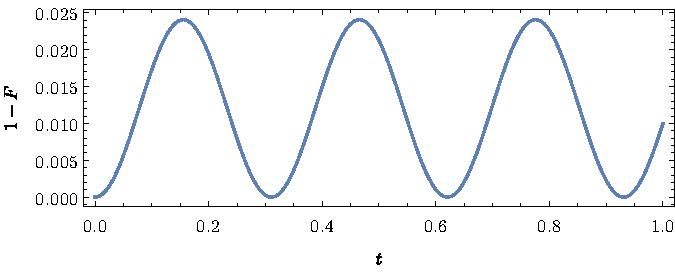
\includegraphics[scale=1.2]{../img/infidelityTimePlotGeod.pdf}
    \caption{Infidelity in time for final time $T_f=1$ for geodesical driving.}
  \label{fig:infidelityTimePlot}
\end{figure}

\vspace{-10pt}\begin{figure}[H]
    \centering
    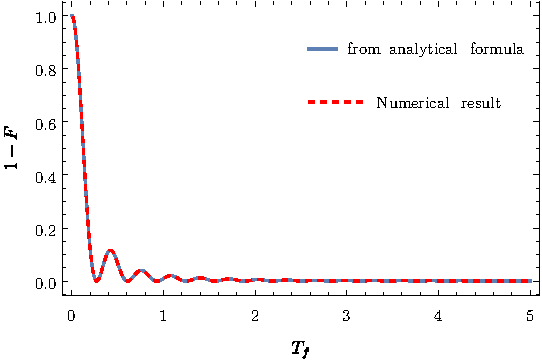
\includegraphics[scale=1.2]{../img/infidelityTfPlot.pdf}
    \caption{Final infidelity dependence on final time $T_f$ for geodesical driving.}
    \label{fig:infidelityTfPlot}
\end{figure}

\begin{figure}[H]
    \centering
    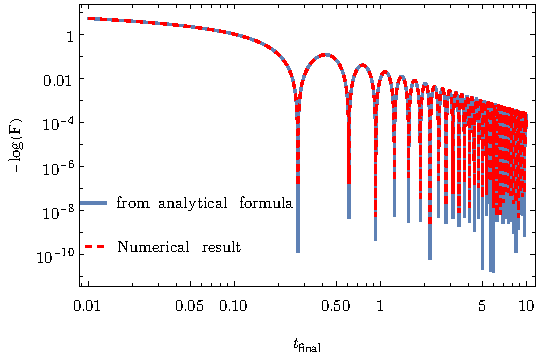
\includegraphics[scale=1.2]{../img/infidelityTfPlotLog.pdf}
    \caption{Infidelity dependence on final time in log-log scale. We can observe difference in numerical evaluation of different firmulas in the height of spikes.}
    \label{fig:infidelityTfPlotLog}
\end{figure}



From the fidelity Eq. \ref{eq:fidelitySimplified} goes that $F=1$ is equivalent to
\begin{equation}
    \cos \left(\sqrt{T_s^2+\pi ^2}\right)=1,
\end{equation}
for $T_s\coloneqq 2sT_f$. The solution to this equation is
\begin{equation}
    T_s=\sqrt{(2 \pi  k)^2-\pi ^2} \text{  for }k\in \mathbb{N}.
    \label{eq:solutionT}
\end{equation}
This can be checked numerically, see Fig. \ref{fig:fidelityZeros}. Because $F=1$ has solutions \ref{eq:solutionT}, its dependence on final time in logarithmic scale has spikes going to $0$, see Fig. \ref{fig:infidelityTfPlotLog}, and their density is linear in $T_f$.
\begin{figure}[H]
    \centering
    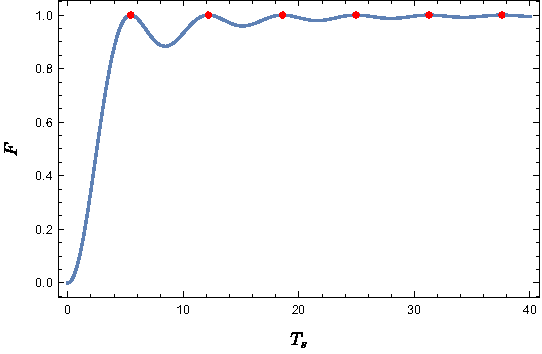
\includegraphics[scale=1.2]{../img/fidelityZeros.pdf}
    \caption{Rescaled final infidelity $T_s\coloneqq 2s T_f$ dependence on final time. Red points are for $F=1$.}
    \label{fig:fidelityZeros}
\end{figure}


Fidelity as a function of time and final time can be seen in Figures \ref{fig:dens3}. Note that only $t<T_f$ has physical meaning.

\begin{figure}[H]
    \centering
    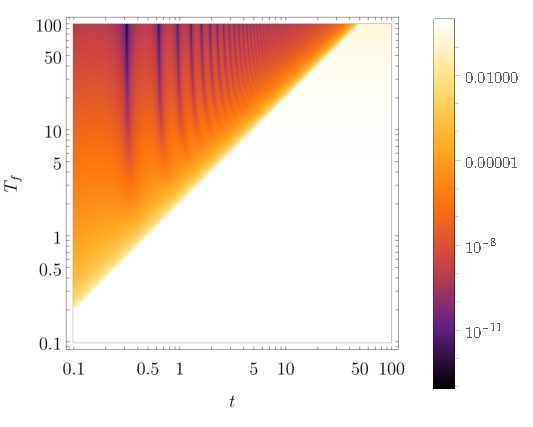
\includegraphics[scale=1.2]{../img/dens3.pdf}
    \caption{Fidelity dependence on time and final time in log log scale. Note that only $t<T_f$ has physical meaning.}
    \label{fig:dens3}
\end{figure}

\subsection{Energy variance}
Evaluating the fidelity for geodesical driving gives a function of time $t$ and final time $T_f$
\begin{equation}
    \begin{split}        
        \delta E^2 =& \frac{s^2}{2 q^2}\Bigg[\Big[16 s^4+2 s^2 \left(\left(\omega ^2-8 s^2\right) \cos (2 t \omega )-8 \omega ^2 \cos ^2(t \omega ) \cos \left(t \sqrt{q}\right)\right)\\
        &+14 s^2 \omega ^2+\omega ^4\Big] -\omega ^2 \left(\left(2 s^2+\omega ^2\right) \cos (2 t \omega )-2 s^2\right) \cos \left(2 t q\right)\\
        & +8 s^2 \omega  q \sin (2 t \omega ) \sin \left(t q\right) + \omega ^3 q \sin (2 t \omega ) \sin \left(2 t q\right) \Bigg],
\end{split}
\end{equation}
see the definition of $q$ under Eq. \ref{eq:evolutionBlue}. It's value as can be seen on Fig. \ref{fig:densVar}. Note that only $t<T_f$ has a physical meaning, therefore the dependence is smooth along the whole geodesical driving protocols.

\begin{figure}[H]
    \centering
    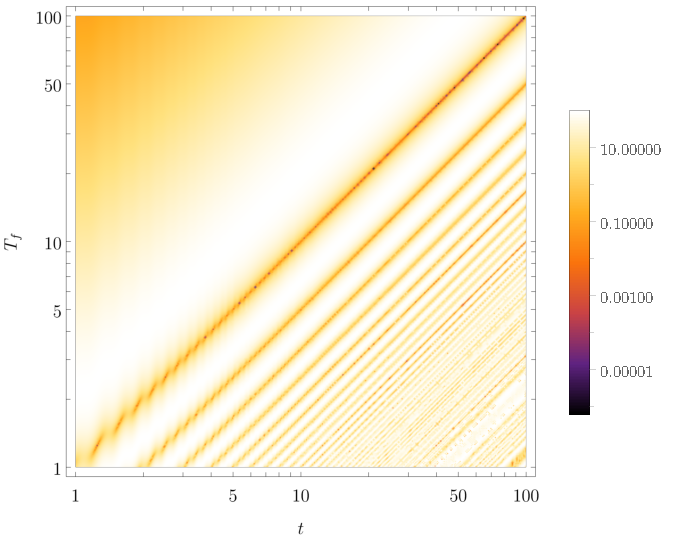
\includegraphics[scale=1.2]{../img/densVar.pdf}
    \caption{Energy variance for geodesical driving protocol.}
    \label{fig:densVar}
\end{figure}

\newpage 
\section{Linear driving}
Another analytically solvable driving is of type 
\begin{equation}
    \Omega(t)=\Omega_{sc}\left(\frac{2t}{T_f}-1\right),\quad \Delta(t)=\Delta_{sc}, \;\;\text{ for } \Omega_{sc}=10, \Delta_{sc}=1,
    \label{eq:linearDrivingdef}
\end{equation}
see Fig. \ref{fig:driving}. Corresponding differential equation of second order is
\begin{equation}
    a''(t)+\left[\frac{2\Omega_{sc}}{T_f}t+ i\frac{2\Omega_{sc}}{T_f}+\Delta_{sc}-\Omega_{sc}\right] a(t)=0,
\end{equation}
with Parabolic Cylinder solution\footnote{https://mathworld.wolfram.com/ParabolicCylinderFunction.html}, see report from Felipe. 
\begin{figure}[H]
    \centering
    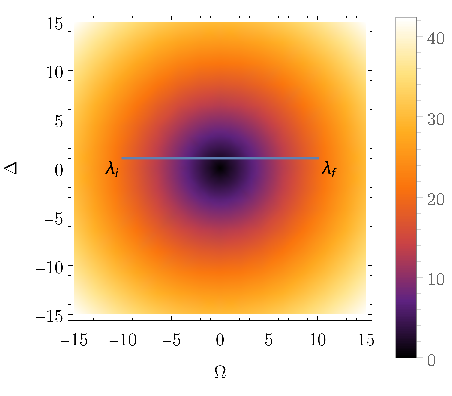
\includegraphics[scale=1.2]{../img/drivingLin.pdf}
    \caption{Driving along the linear path. $\lambda_i=(-10;1)$ and $\lambda_f=(10;1)$ are initial resp. final parameters. DensityPlot shows the difference between Hamiltonian eigenvalues.}
    \label{fig:driving}
\end{figure}

From linear driving definition \ref{eq:linearDrivingdef} and energy dependence \ref{eq:energy} we have
\begin{equation}
    \dot \Delta(t)=0;\quad \Delta(t) \overset{\textcolor{gray}{\Delta(t)>0}}{=} \sqrt{\frac{E^2_{dif}(t)}{4}-\Omega^2(t)};\quad E_{dif}\coloneqq E_1-E_0.
\end{equation}
Substituting to functions from the Harmonic oscillator (Eq. \ref{eq:gammaDef}, \ref{eq:frequency}) we get 
\begin{align}
    \gamma(t) &= 0\\
    \omega^2(t)&=i\frac{2\Omega_{sc}}{T_f}+\frac{\Omega_{sc}}{4}\left(\frac{2t}{T_f}-1\right)^2+\frac{\Delta_{sc}^2}{4}=i\frac{2\Omega_{sc}}{T_f}+\frac{E^2_{dif}(t)}{4}\label{eq:oscillationsLinear}
\end{align}


\subsection{Dependence on time}
The fidelity in time can be seen on Fig. \ref{fig:infidelityTimePlotLin}. For $t\approx T_f/2$ Hamiltonian parameters change quickly which leads to fast state excitation. Then the Harmonic oscillator damping gets involved and oscillations are quickly going to zero, never disappearing entirely.

We can see that the final fidelity decreases with longer final time, which correctly leads to adiabatic driving $\lim_{T_f\rightarrow \infty} F=0$. For short final times we can observe so called quench, $\lim_{T_f\rightarrow 0} F=1$. The interesting phenomenon on this image are the oscilations around $t=T_f/2$, which have gigher relative amplitude to the final infidelity and bigger frequency with longer final time. 

\begin{figure}[H]
    \centering 
    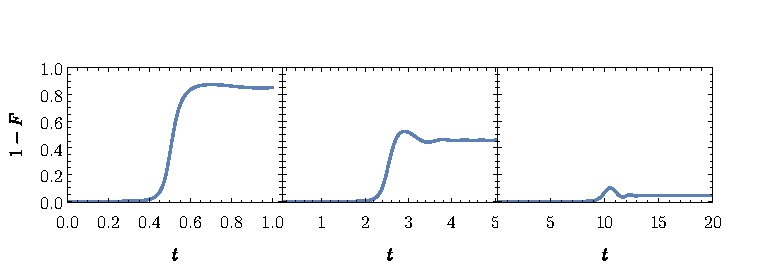
\includegraphics[scale=1.185]{../img/infidelityInTimePlot1.pdf}
    \caption{Infidelity in time for three final times $T_f\in\{1,5,20\}$ for the linear driving.}
  \label{fig:infidelityTimePlotLin}
\end{figure}


\subsection{Final fidelity}
Because the oscillations after fast parameter change in the Hamiltonian never disappear entirely, we must observe those oscillations even at the final time. \emph{Final fidelity} (meaning the fidelity at final time $T_f$) has dependence on $T_f$ as can be seen in Fig. \ref{fig:infidelityTfPlotLogLinCombined}. Because after the final time $T_f^{\Delta_{sc}=1}\approx 120$ the values are so small, we can observe some fine structure of the fidelity, along with numerical error artifacts.
\begin{figure}[H]
    \centering
    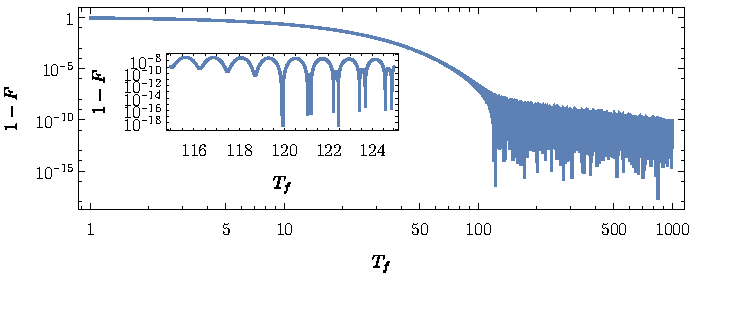
\includegraphics[scale=1.2]{../img/infidelityTfPlotLogLinCombined1.pdf}
    \caption{Final infidelity as a function of $T_f$ with zoom on transitional part.}
    \label{fig:infidelityTfPlotLogLinCombined}
\end{figure}

First of all, the numerical precision of this calculation was found to be around $10^{-14}$. This means that the oscillations we see on Fig. \ref{fig:infidelityTfPlotLogLinCombined} are of physical origin with some additional numerical error. In fact these small oscillations are the remnants of the fast excitation during close approach of energy levels, see Fig. \ref{fig:infidelityTimePlotLin}. One would like to analyze these oscillations from $\omega^2(t)$ described by Eq. \ref{eq:oscillationsLinear}. The problem is that we are observing the fidelity $F=\braket{0(t)|\psi(t)}$ where $\bra{0(t)}\neq const.$ and is described by Eq. \ref{eq:eigenvectors}. This value of first element of ground state vector $\ket{0(t)}^1$ starts at value close to $0$ and around $t=T_f/2$ slowly changes and becomes almost $1$, see Fig. \ref{fig:zeroState}.
\begin{figure}[H]
    \centering
    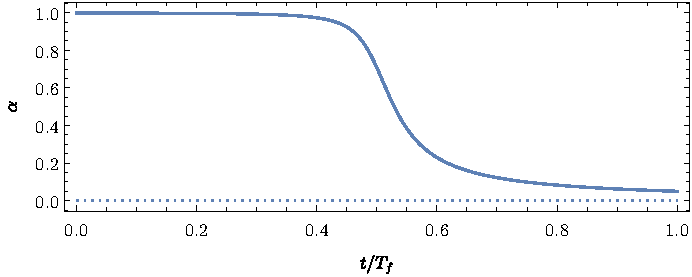
\includegraphics[scale=1.2]{../img/zeroState.pdf}
    \caption{Value of first element of the ground state vector $\ket{0(t)}^1$ during linear driving.}
    \label{fig:zeroState}
\end{figure}


This means that at the end of the driving (for definitions see Eq. \ref{eq:eigenvectors})\footnote{Even thought kets are vectors, we are forced to write indices down to avoid confusion with powers.}
\begin{equation}
   \frac{1}{N_+} \ket{0(t)}_1=\frac{E_0(t)+\Omega(t)}{\Delta(t)}\gg 1 =\frac{1}{N_+} \ket{0(t)}_2.
\end{equation}
Writing $\ket{\psi(t)}\eqqcolon (a(t),b(t))$, we get the fidelity approximation at the end of driving
\begin{equation}
    F_{end}= \left|N_+ \left(
        \frac{E_0(t)+\Omega(t)}{\Delta(t)} a(t)+b(t)
        \right)\right|^2 \approx a^2(t).
\end{equation}
Therefore when $t$ is getting close to $T_f$ the fidelity is oscilating with frequency \ref{eq:frequency}.


We can eliminate the effect of oscillations by averaging over time. For that we define the \emph{average final infidelity}
\begin{equation}
    \langle 1-F\rangle_p(T_f) \coloneqq \frac{1}{(1-p) T_f}\int_{p T_f}^{T_f} F(t)\d t.
\end{equation}
It turned out that averaging over 1 \% or 10 \% of the drivine (i.e. taking $\langle 1-F\rangle_{0.9}$, resp $\langle 1-F\rangle_{0.99}$) gave approximately the same results for long enough drivings. The result can be seen on Fig. \ref{fig:infidCombined}.

Using this we can describe the driving using three regimes\footnote{The coefficient $p$ is assumed to be small enough not to cover the biggest oscillations after $t=T_f/2$ and big enough to average over suffitient number of oscillations. $p\tilde\in[0.6T_f,0.999T_f]$}:
\begin{itemize}
    \item \emph{exponential/fast-driving regime} -- $\langle 1-F\rangle_p= \exp(-\xi T_f)$, $\xi\in\R^+$
    \item \emph{transitional regime} -- happens around \emph{critical time} $T_c$. \textcolor{red}{smoothening is not enough to remove the oscillations}
    \item \emph{polynomial/close-adiabatic regime} -- $\langle 1-F\rangle_p\propto T_f^{-\kappa}$ for $\kappa\in \R^+$.
\end{itemize}

\begin{figure}[H]
    \centering
    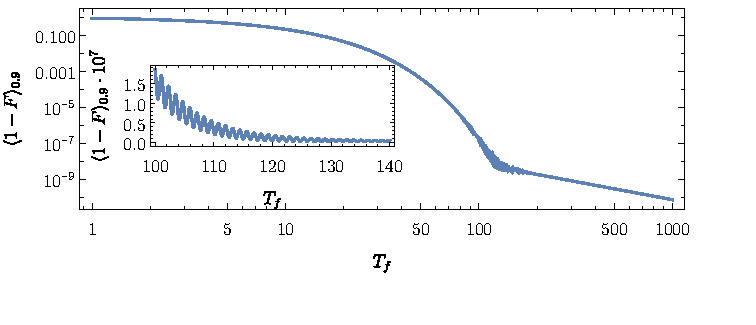
\includegraphics[scale=1.2]{../img/infidCombined1.pdf}
    \caption{Final infidelity as a function of $T_f$ in log log scale wit linear scaled plot inserted.}
    \label{fig:infidCombined}
\end{figure}


The reason for different behavior in slow and fast driving protocols comes from the fact that oscillations do not dissapear entirely for $t=T_f$. By comparing the infidelity for $t$ close to $T_f$, Fig. \ref{fig:undercritical}, \ref{fig:overcritical}, we see that for $T_f<T_c$ the oscillations are smaller than the final infidelity and $1-F\neq 0$. For $T_f>T_c$ the oscillations amplitude is bigger than final infidelity.

\begin{figure}[H]
    \centering
    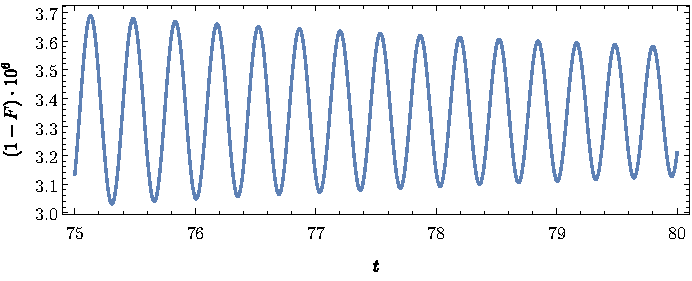
\includegraphics[scale=1.2]{../img/undercritical.pdf}
    \caption{Final infidelity as a function of $T_f$ for fast-driving regime.}
    \label{fig:undercritical}
\end{figure}

\begin{figure}[H]
    \centering
    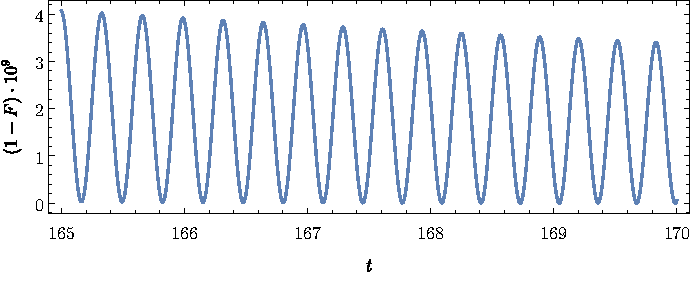
\includegraphics[scale=1.2]{../img/overcritical.pdf}
    \caption{Final infidelity as a function of $T_f$ for close-adiabatic regime.}
    \label{fig:overcritical}
\end{figure}

Two questions now arise. What are the coefficients $\xi$ and $\kappa$ and on which intervals in $T_f$ these transitions hold? 

\subsection{Critical time $T_c$}
The critical time $T_c$ is the point where the fidelity dependence on final time becomes polynomial. We have showed that for 
\begin{equation}
    \text{for}\begin{cases}
        T_f<T_c \\
        T_f>T_c 
    \end{cases}\text{the oscillations amplitude } A \text{ is }
    \begin{cases}
        A<1-F_{final}\\
        A>1-F_{final}
    \end{cases}.
\end{equation}
On Fig. \ref{fig:dens2} we can see the dependence of critical time as the point of transition between \emph{smooth} and \emph{chaotic} regimes, on $\Delta=\Delta_sc$ for the linear driving. The fine structure, see Fig. \ref{fig:dens2Zoom}, is caused by the oscillatory character of the final fidelity. The approximated dependence is
\begin{equation}
    T_c\tilde\propto \Delta_{sc}^{-2}
\end{equation}


\begin{figure}[H]
    \centering 
    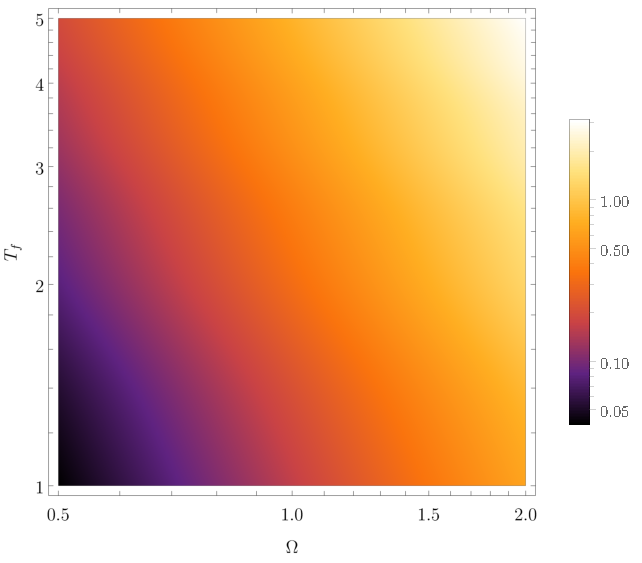
\includegraphics[scale=1.2]{../img/dens2.pdf}
    \caption{Final infidelity as a function of $\Delta$ and $T_f$ and its three regimes. Zoomed boundary between them can be seen on \ref{fig:dens2Zoom}.}
    \label{fig:dens2}
\end{figure}

\begin{figure}[H]
    \centering 
    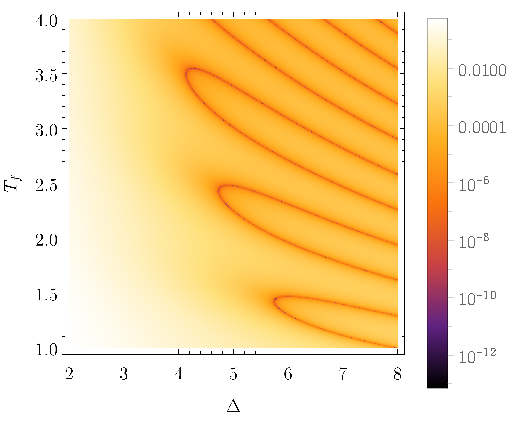
\includegraphics[scale=1.2]{../img/dens2Zoom.pdf}
    \caption{Fine structure of the boundary between fast-driving and adiabatic regimes of final infidelity.}
    \label{fig:dens2Zoom}
\end{figure}


\subsection{Coefficients $\xi$ and $\kappa$}
TODO

\newpage
\subsection{Energy variance}
Energy variance resembles structure similar to fidelity. Compare Fig. \ref{fig:densVariance} with \ref{fig:dens3}. 
\begin{figure}[H]
    \centering
    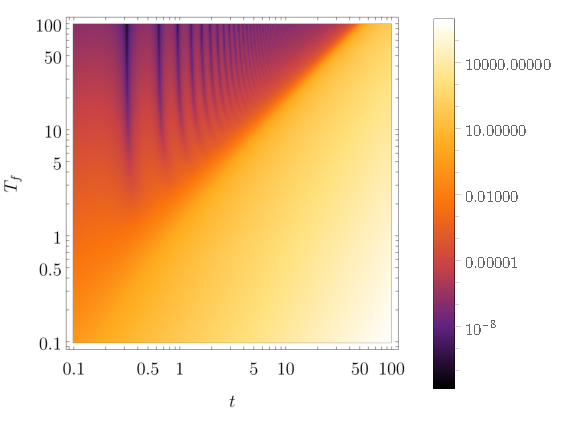
\includegraphics[scale=1.2]{../img/densVariance.pdf}
    \caption{Energy variance for $\Delta_{sc}=0.2$ for linear driving. Note that only $t<T_f$ has physical meaning.}
    \label{fig:densVariance}
\end{figure}

\begin{figure}[H]
    \centering
    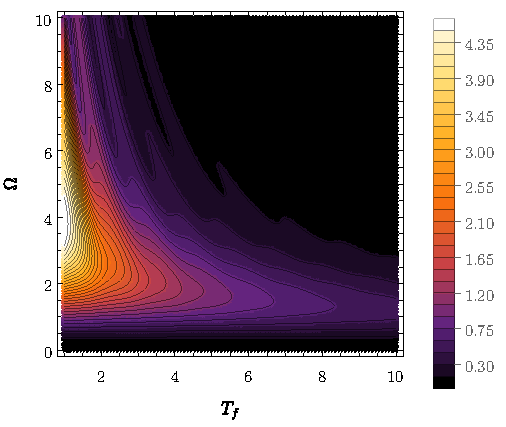
\includegraphics[scale=1.2]{../img/contVariance.pdf}
    \caption{Energy variance for $t=T_f/2$ for linear driving.}
    \label{fig:densVarLin}
\end{figure}

















\section{Energy variance for two level system}
For two level system, the variance
\begin{equation}
    \delta E^2(t)\coloneqq \braket{\psi(t)|\HH^2|\psi(t)}-\braket{\psi(t)|\HH|\psi(t)}^2
\end{equation}
can be rewritten inserting identity $\textcolor{purple}{\Id=\ket{0}\bra{0}+\ket{1}\bra{1}}$ around Hamiltonian. Omitting the time dependence of every element we get
\begin{equation}
    \begin{split}
        \delta E^2 =& \braket{\psi|\textcolor{purple}{\Id}\HH^2\textcolor{purple}{\Id}|\psi}-\braket{\psi|\textcolor{purple}{\Id}\HH\textcolor{purple}{\Id}|\psi}^2\\
        =&\braket{\psi|0}\braket{0|\HH^2|0}\braket{0|\psi}+\braket{\psi|1}\braket{1|\HH^2|1}\braket{1|\psi}\\
        +&\textcolor{gray}{\braket{\psi|0}\braket{0|\HH^2|1}\braket{1|\psi}+\braket{\psi|1}\braket{1|\HH^2|0}\braket{0|\psi}}\\
        -&\Big(\braket{\psi|0}\braket{0|\HH|0}\braket{0|\psi}+\braket{\psi|1}\braket{1|\HH|1}\braket{1|\psi}\\
        +&\textcolor{gray}{\braket{\psi|0}\underbrace{\braket{0|\HH|1}}_{\propto \braket{0|1}=0}\braket{1|\psi}+\braket{\psi|1}\underbrace{\braket{1|\HH|0}}_{\propto \braket{0|1}=0}\braket{0|\psi}}\Big)^2.
    \end{split}
\end{equation}
Using Fidelity definition $F(t)=\left|\braket{0(t)|\psi(t)}\right|^2$ and Schr\"odinger equation $\HH\ket{k}=E_k\ket{k}$ we have
\begin{equation}
    \delta E^2 = FE_0^2+(1-F)E_1^2 - (FE_0+(1-F)E_1)^2 = F(1-F)(E_0-E_1)^2.
\end{equation}
For three level system we have $\textcolor{purple}{\Id=\ket{0}\bra{0}+\ket{1}\bra{1}+\ket{2}\bra{2}}$ and
\begin{equation}
    \delta E^2=\sum_{k=1}^3 E_k^2 F_k(1-F_k)-4\prod_{k=1}^3 E_kF_k-2F_0F_1E_0E_1-2F_0F_2E_0E_2-2F_1F_2E_1E_2,
\end{equation}
for $F_k\coloneqq \braket{k|\psi}$, which has no practical simplification.
